\chapter{Dataset}
\label{appendixD}
\thispagestyle{empty}

\noindent In this appendix we report the most significant parts of our dataset.

\vspace{0.5cm}

\section{C1 and C0 Training samples}

\label{appendixD:samples}

The training set is composed of 216 images for each of the two classes. Here we show some training samples for both classes.
Figure \ref{appendixD:fig1} contains a subset of \textbf{C1} image patches, and Figure \ref{appendixD:fig2} contains a subset of \textbf{C0} samples.


\begin{figure}[!hb]
 \centering
  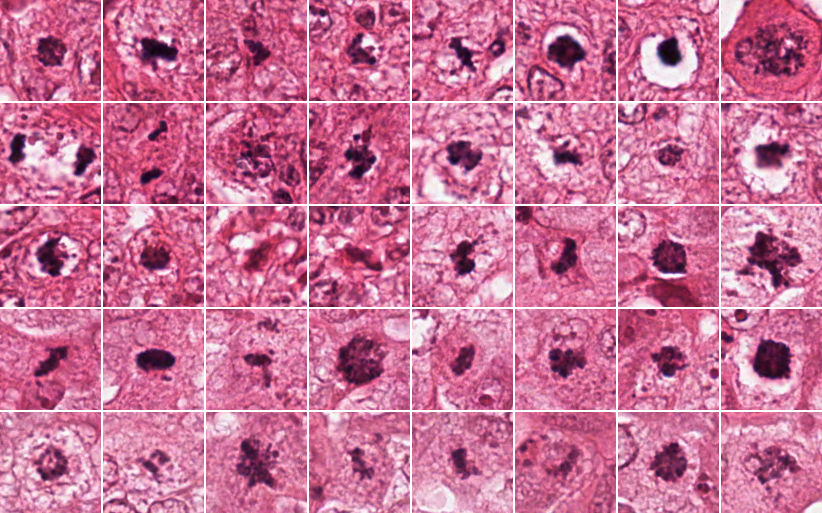
\includegraphics[width=0.96\textwidth]{./images/dataset/posTrainDataSet.png}
  \caption{Examples of \textbf{C1} training images}
  \label{appendixD:fig1}
\end{figure}

\begin{figure}[!ht]
 \centering
  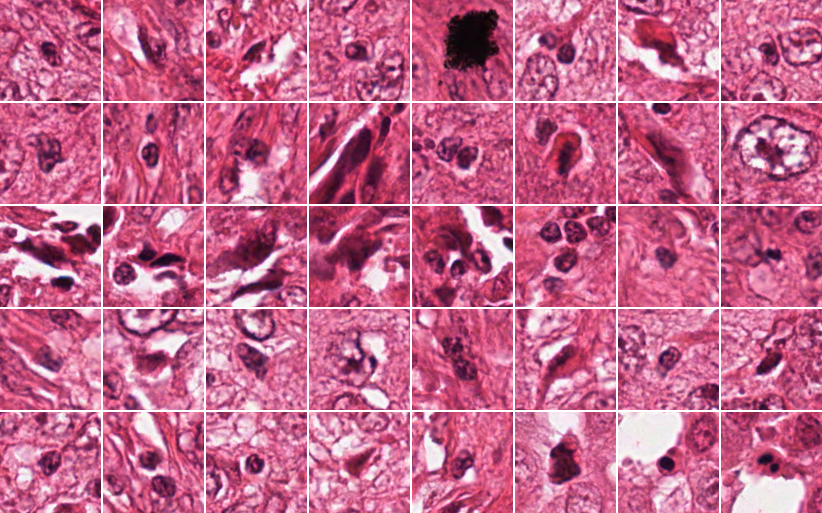
\includegraphics[width=0.96\textwidth]{./images/dataset/negTrainDataSet.png}
  \caption{Examples of \textbf{C0} training images}
  \label{appendixD:fig2}
\end{figure}

\vspace{1.5cm}

\section{C1 and C0 Evaluation samples}

\label{appendixD:h_diff}

The evaluation set is composed of 87 images for each of the two classes. In Chapter \ref{chapter6} we divided the evaluation dataset in three
subsets, corresponding to \textit{easy}, \textit{medium} and \textit{hard} samples in function of the ability of our test subjects to correctly
classify them (see Section \ref{ch6:diff1}).

\begin{figure}[!hb]
 \centering
  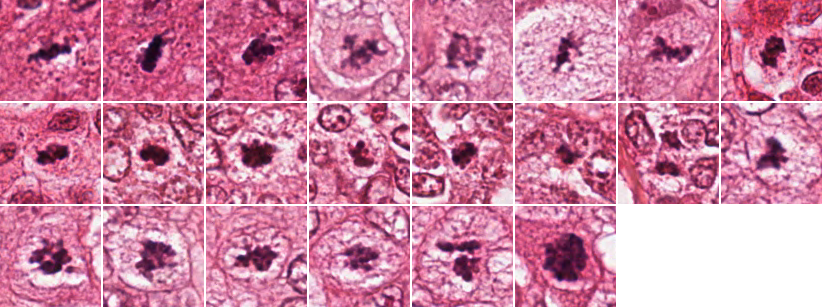
\includegraphics[width=0.96\textwidth]{./images/dataset/C1_easy.png}
  \caption{\textit{Easy} \textbf{C1} evaluation images}
  \label{appendixD:fig3}
\end{figure}

\clearpage

\begin{figure}[!ht]
 \centering
  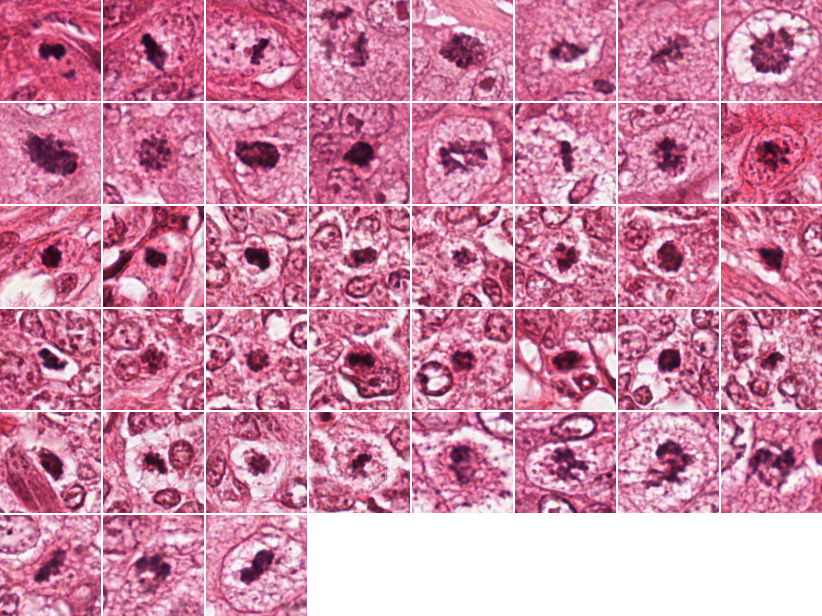
\includegraphics[width=0.96\textwidth]{./images/dataset/C1_med.png}
  \caption{\textit{Medium} \textbf{C1} evaluation images}
  \label{appendixD:fig4}
\end{figure}

Samples are divided so that \textit{easy} subset contains the first 25\% of the samples (Figure \ref{appendixD:fig3}), \textit{hard} subset the last 25\%
(Figure \ref{appendixD:fig5}) and the \textit{medium} the remaining 50\% (Figure \ref{appendixD:fig4}).

\begin{figure}[!hb]
 \centering
  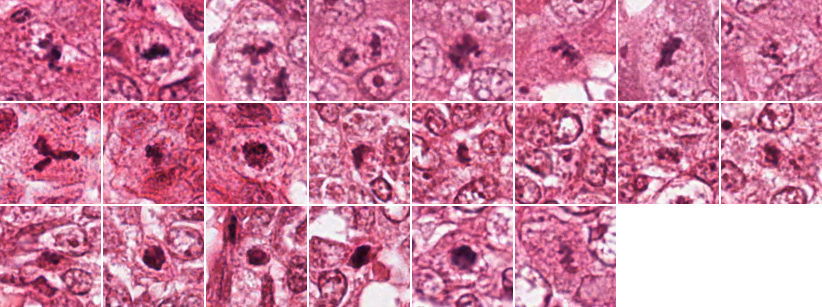
\includegraphics[width=0.96\textwidth]{./images/dataset/C1_hard.png}
  \caption{\textit{Hard} \textbf{C1} evaluation images}
  \label{appendixD:fig5}
\end{figure}

\clearpage

\begin{figure}[!ht]
 \centering
  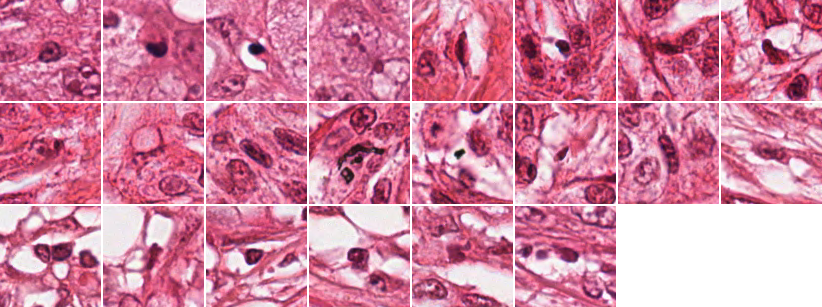
\includegraphics[width=0.96\textwidth]{./images/dataset/C0_easy.png}
  \caption{\textit{Easy} \textbf{C0} evaluation images}
  \label{appendixD:fig6}
\end{figure}

Also for \textbf{C0} class, samples are divided so that \textit{easy} subset contains the first 25\% of the samples (Figure \ref{appendixD:fig6}), \textit{hard} subset the last 25\%
(Figure \ref{appendixD:fig8}) and the \textit{medium} the remaining 50\% (Figure \ref{appendixD:fig7}).


\begin{figure}[!hb]
 \centering
  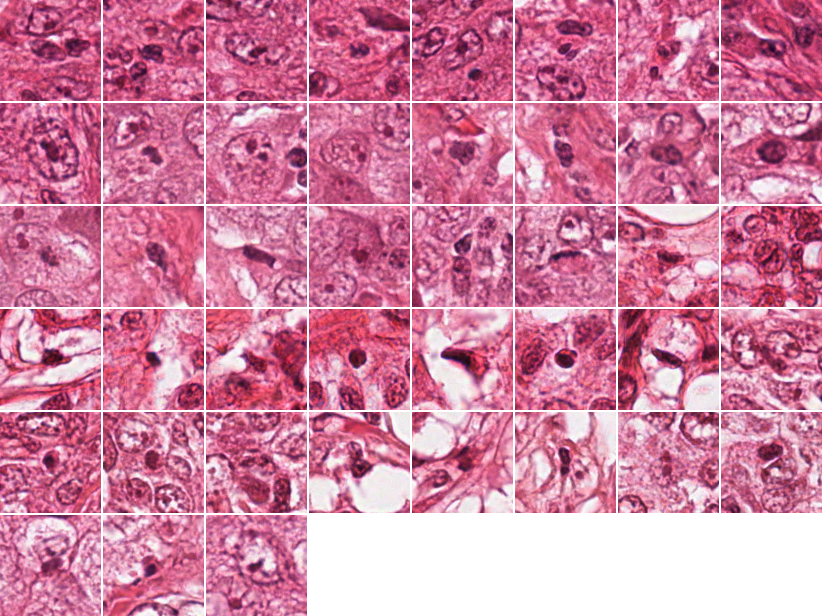
\includegraphics[width=0.96\textwidth]{./images/dataset/C0_med1.png}
  \caption{\textit{Medium} \textbf{C0} evaluation images}
  \label{appendixD:fig7}
\end{figure}

\clearpage

\begin{figure}[!ht]
 \centering
  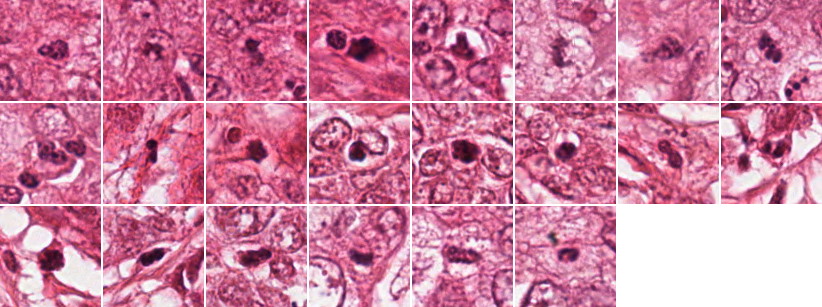
\includegraphics[width=0.96\textwidth]{./images/dataset/C0_hard.png}
  \caption{\textit{Hard} \textbf{C0} evaluation images}
  \label{appendixD:fig8}
\end{figure}


\vspace{0.5cm}

\section{Classifier Difficulties}

\label{appendixD:cl_diff}
In Section \ref{ch6:sec_class} we compared the performances of our best classifiers with test subjects and analyzed if some samples were particularly
difficult (i.e. many classifiers are not able to label them correctly). We considered the 8 best classifiers (4 \Glspl{RF} and 4 \Glspl{SVM})
and considered mis-labeled samples by at least 5 classifiers. The next two images show the most difficult examples. Each patch reports the \textit{human difficulty} (see
Section \ref{appendixD:h_diff} and Section \ref{ch6:diff1}) and the frequency of errors (i.e. how many classifiers mis-labeled the image:
\textit{f} on each title of Figure \ref{appendixD:fig9} and Figure \ref{appendixD:fig10}).

\begin{figure}[!hb]
 \centering
  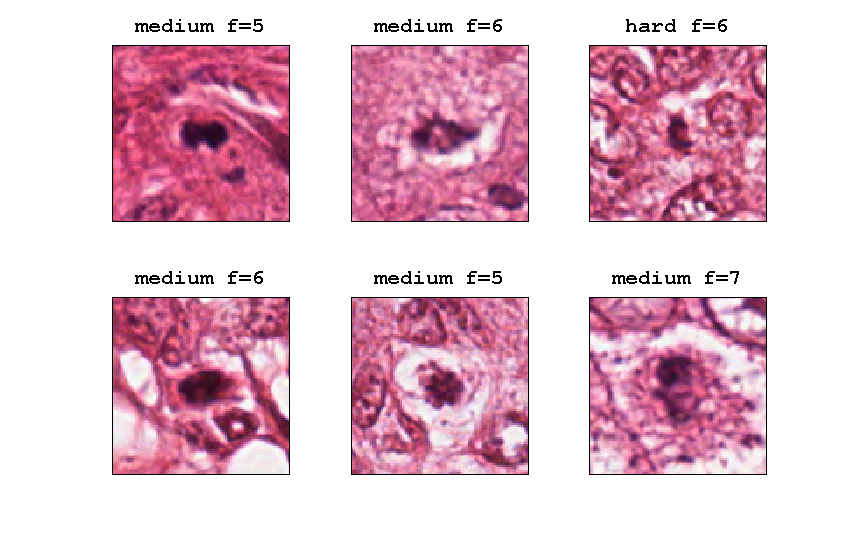
\includegraphics[width=0.72\textwidth]{./images/dataset/classFN.png}
  \caption{RF and SVM classifiers: Mis-labeled \textbf{C1} evaluation images}
  \label{appendixD:fig9}
\end{figure}

\clearpage

\begin{figure}[!ht]
 \centering
  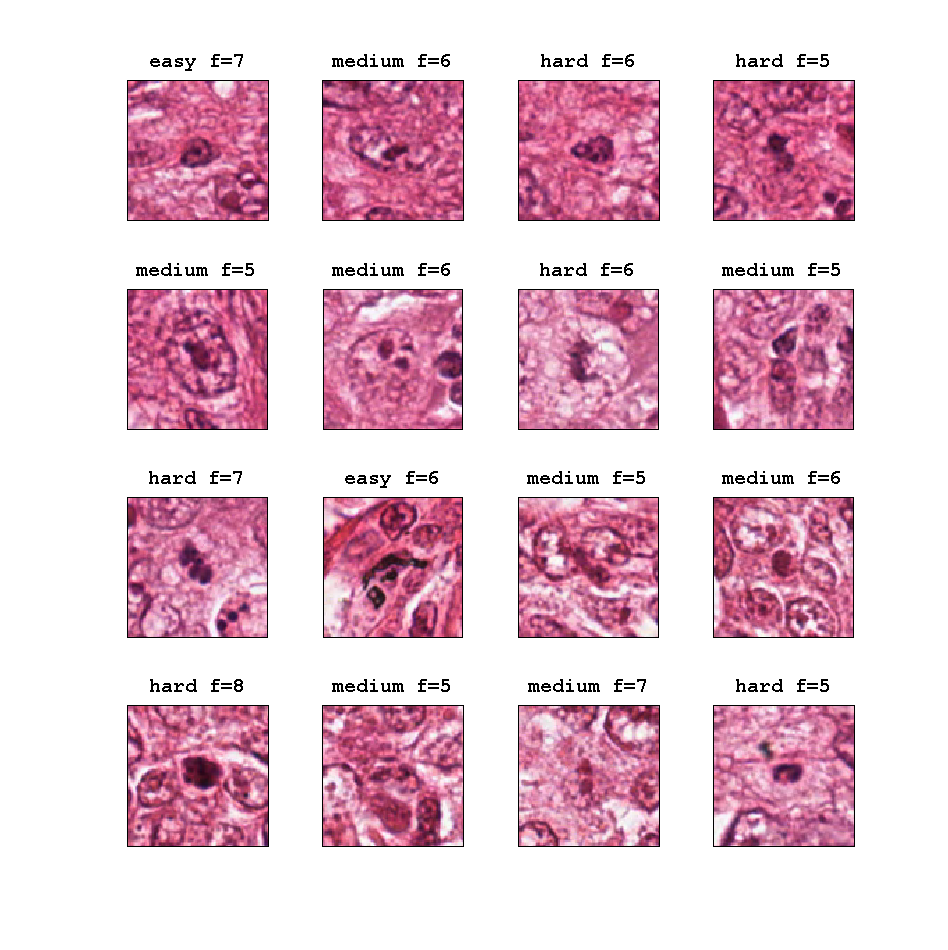
\includegraphics[width=0.94\textwidth]{./images/dataset/classFP.png}
  \caption{RF and SVM classifiers: Mis-labeled \textbf{C0} evaluation images}
  \label{appendixD:fig10}
\end{figure}

